% presentar o problema que se vai tratar, incluír o obxectivo principal e os
% específicos, de ser o caso, do traballo presentado, indicando o alcance para cada un deles.

\section{Objetivos} \label{sec:obj}
    En esta sección se especifican los objetivos que persigue el proyecto presentado. Se incluyen tanto los objetivos principales, donde se describe una solución general que se desea obtener del proceso de desarrollo, como los objetivos específicos donde se detalla qué es lo que se busca en cada una de las partes del sistema.

    \subsection{Principal}
        El objetivo principal que persigue este proyecto es la creación de una herramienta modular que permita, de forma automatizada, obtener periódicamente información de los sistemas y funcionalidades que deban ser monitorizados en cada uno de los servidores \textit{Windows} y servirla a diferentes sistemas de monitorización enfocados en el usuario, que podrán ser utilizados para tomar las medidas oportunas.
        
        Esto representa un gran avance para la situación actual de la monitorización, donde la mayoría de las acciones son tomadas en función de comprobaciones realizadas a mano o mediante el uso de \textit{scripts} que, a pesar de facilitar la obtención de datos relevantes, no están organizados de forma centralizada.
        
        La implantación de un nuevo sistema de monitorización totalmente centralizado se traduce en un ahorro de tiempo y esfuerzo por parte de los administradores de los servidores. Además, proveer una interfaz intuitiva con un panel donde los fallos, actualizaciones pendientes, amenazas, etc. sean fácilmente identificables, permitirá prevenir errores y aplicar las actualizaciones necesarias lo antes posible.
        
    \subsection{Específicos}
        \begin{itemize}
            \item \textbf{Sistema modular:} \\
                El sistema estará compuesto por un agente y varios \textit{plugins}, que ser capaz de gestionar y comunicar, además de proveerlos con las configuraciones necesarias para que realicen funcionalidades específicas.
                
            \item \textbf{Plugins de entrada:} \\
                La información del sistema será recopilada mediante el uso de \textit{plugins de entrada}, los cuales no tendrán un funcionamiento autónomo y estarán centrados en una información específica.
                
            \item \textbf{Plugins de salida:} \\
                Los datos recibidos desde los \textit{plugins de entrada} serán utilizados por los \textit{plugins de salida}, los cuales enviarán la información a los sistemas de gestión de información o la presentarán directamente al usuario.
                
            \item \textbf{Sistema de planificación:} \\
                Los \textit{plugins} se ejecutarán periódicamente a través del \textit{agente}. De esta forma se controlará tanto el orden como la frecuencia de obtención y transmisión de la información.
                  
            \item \textbf{Captura de eventos del sistema:} \\
                El \textit{agente} podrá ser suscrito a los \textit{logs} de eventos del sistema. La información generada en estos \textit{logs} en tiempo real será utilizada por los \textit{plugins de salida} especificados.
            
            \item \textbf{Actualizador automático:} \\
                Tanto el \textit{agente} como los \textit{plugins} deberán ser actualizados automáticamente siempre que haya una nueva versión disponible. El \textit{sistema de planificación} se encargará de que este proceso se realice de forma regular.
                
            \item \textbf{Archivo de configuración:} \\
                Se utilizará un archivo de configuración donde se especifiquen las opciones con las que serán ejecutadas todas las funcionalidades del sistema. Esto incluye tanto el actualizador como los \textit{plugins}, sus períodos de ejecución, y vinculaciones.
                
            \item \textbf{Servicio:} \\
                El sistema podrá ser iniciado como un \textit{Servicio} que se mantenga en ejecución permanentemente en segundo plano. De esta forma podrá llevar a cabo todas las tareas configuradas sin la intervención del usuario. Además, iniciará automáticamente con el arranque del sistema operativo.
                
            \item \textbf{Interfaz de línea de comandos (\textit{CLI}):} \\
                Mediante el uso de una consola de comandos se podrá controlar la instalación y estado del \textit{servicio}. Además, se podrá consultar la información del servidor utilizando un archivo de configuración o especificando manualmente los \textit{plugins} que se desea ejecutar junto con las opciones necesarias para ello. La impresión por pantalla de la información será llevada a cabo por un \textit{plugin de salida} específico, el cual será la salida predeterminada para la \textit{CLI}.
        \end{itemize}


% check this again before start
%\cleardoublepage
%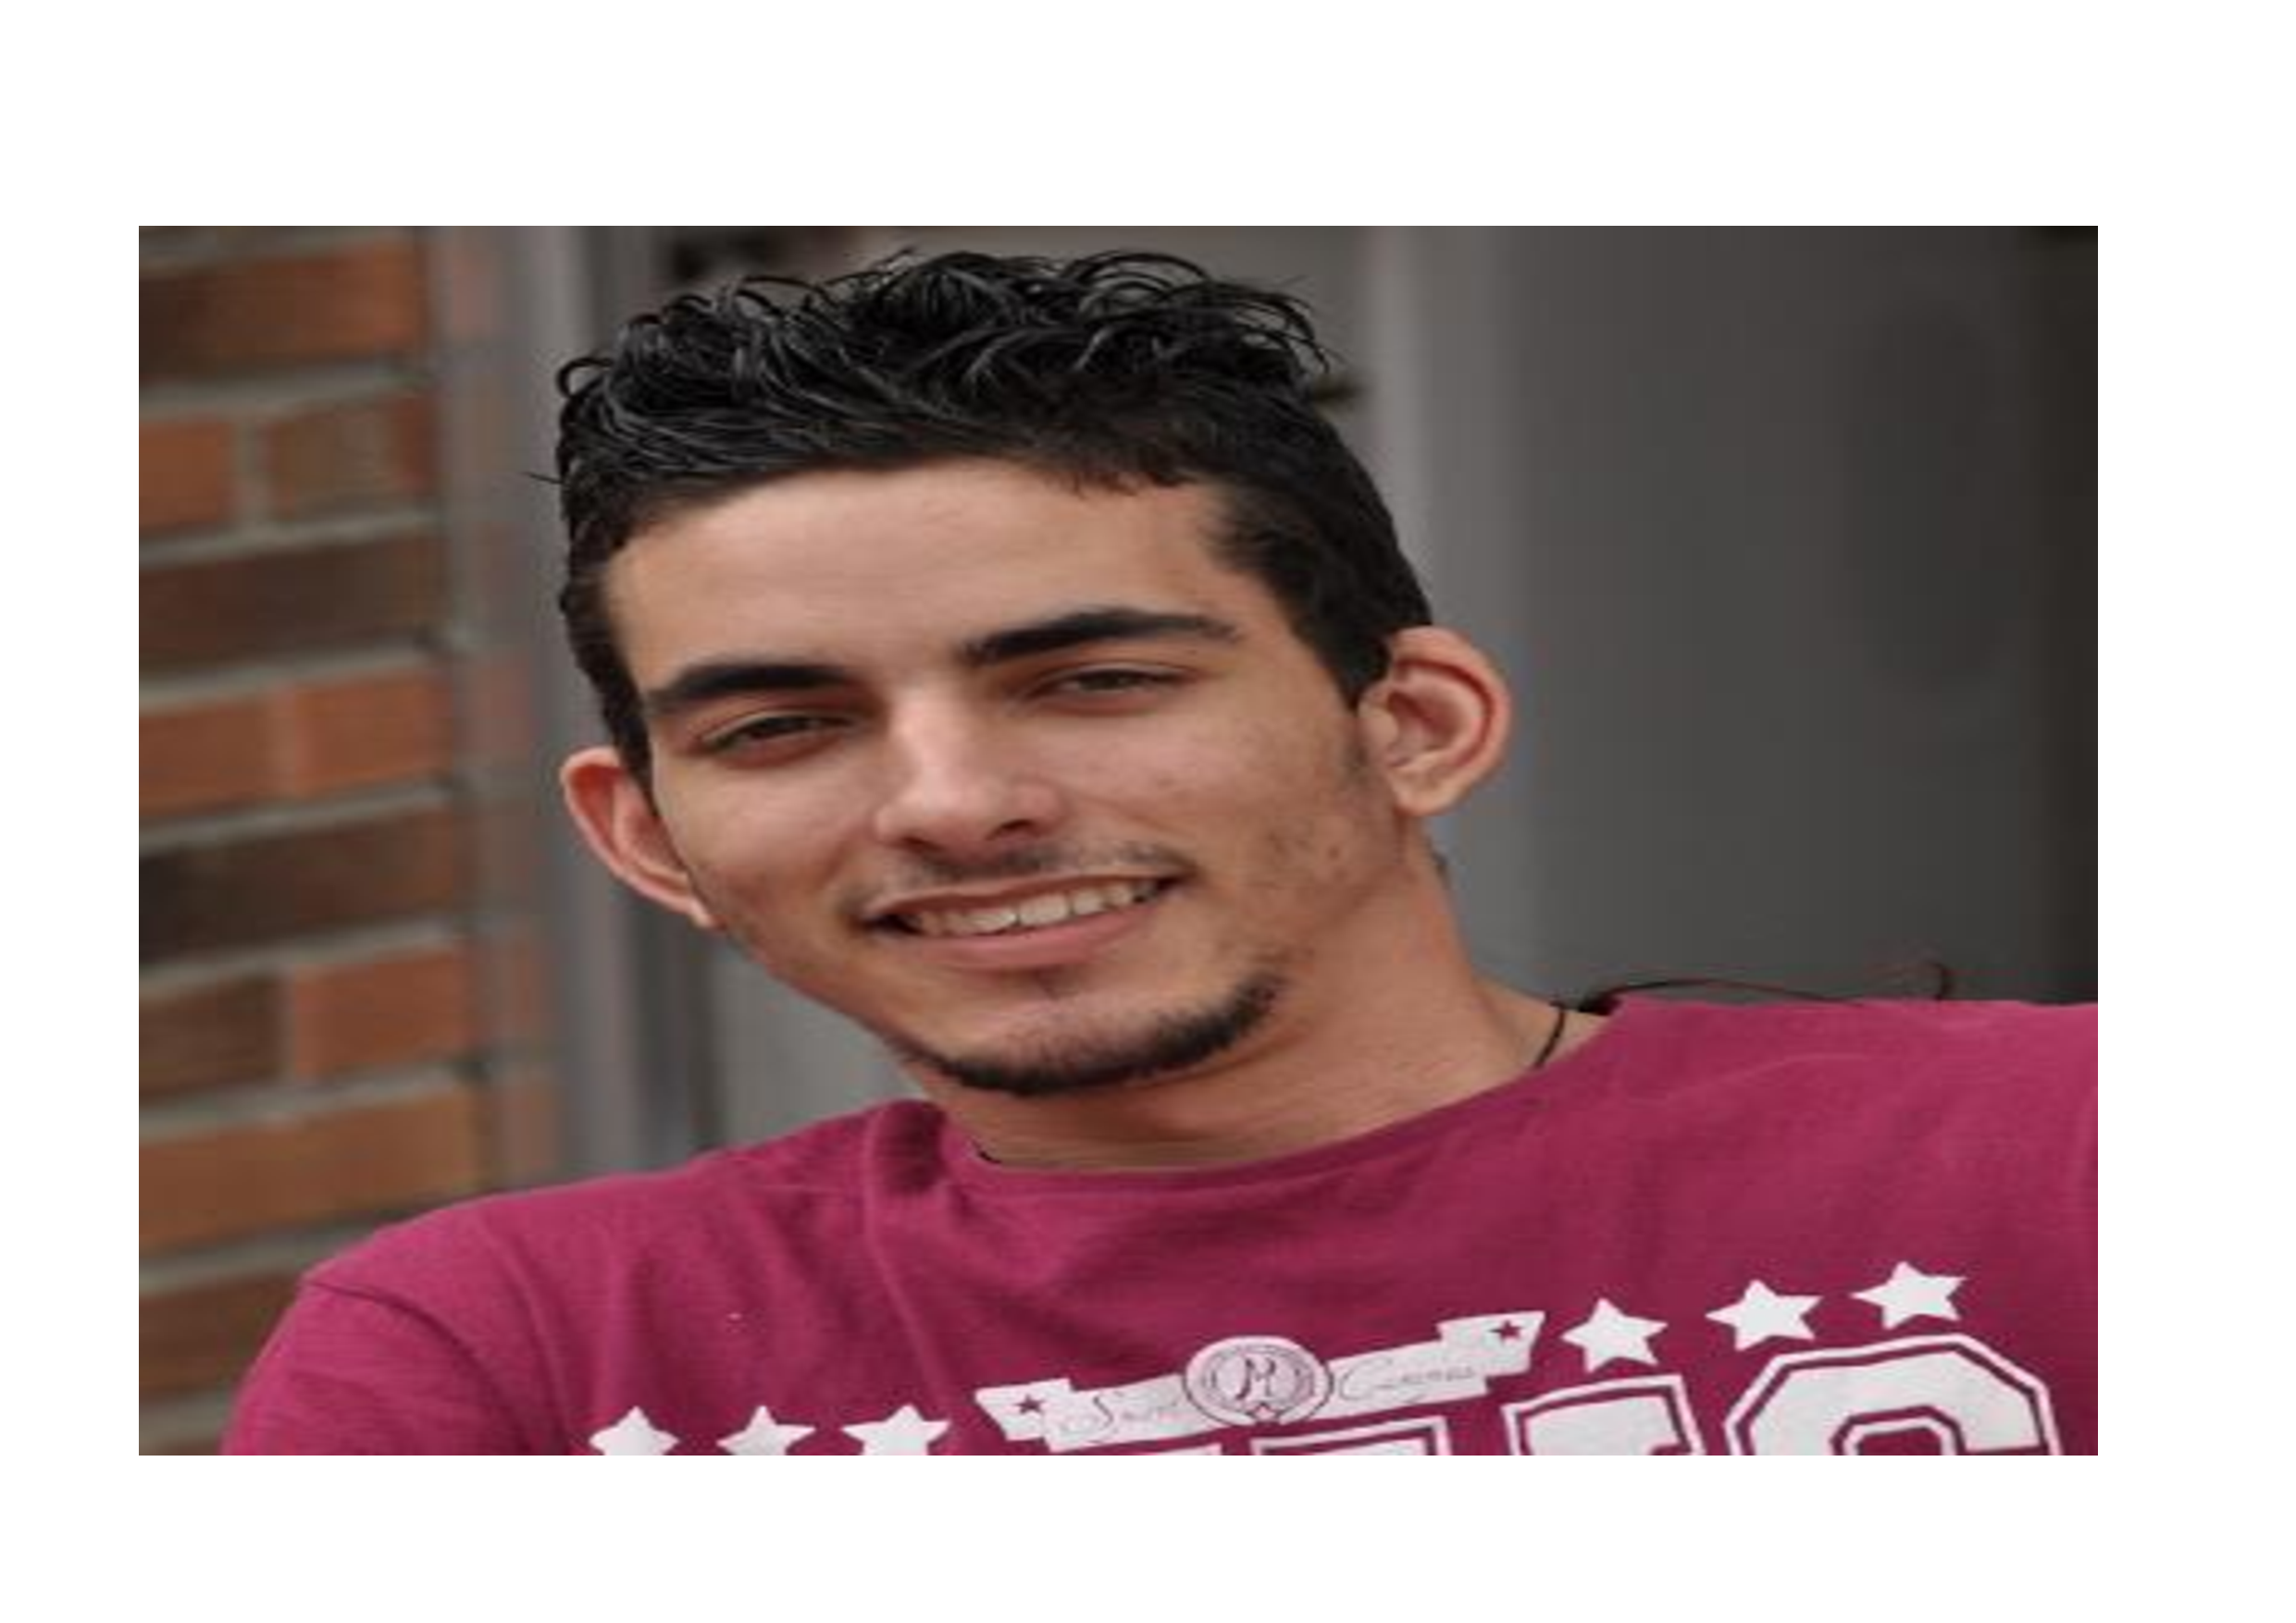
\includepdf[
%    pages=1,
%    fitpaper,
%    addtolist={
%        1,
%        figure,
%        A test figure included with the help of the \texttt{pdfpages} package,
%        fig:test1
%    },
%    pagecommand={\label{fig:test}\thispagestyle{fancy}}
%]{../images/a.pdf}
% TODO: añadir cara trasera a3 después

    